\documentclass[crop,tikz,convert={outext=.svg,command=\unexpanded{pdf2svg \infile\space\outfile}},multi=false]{standalone}[2012/04/13]
%\usetikzlibrary{...}% tikz package already loaded by 'tikz' option
        \newcommand\degree[0]{^{\circ}}
\makeatletter
\begin{document}
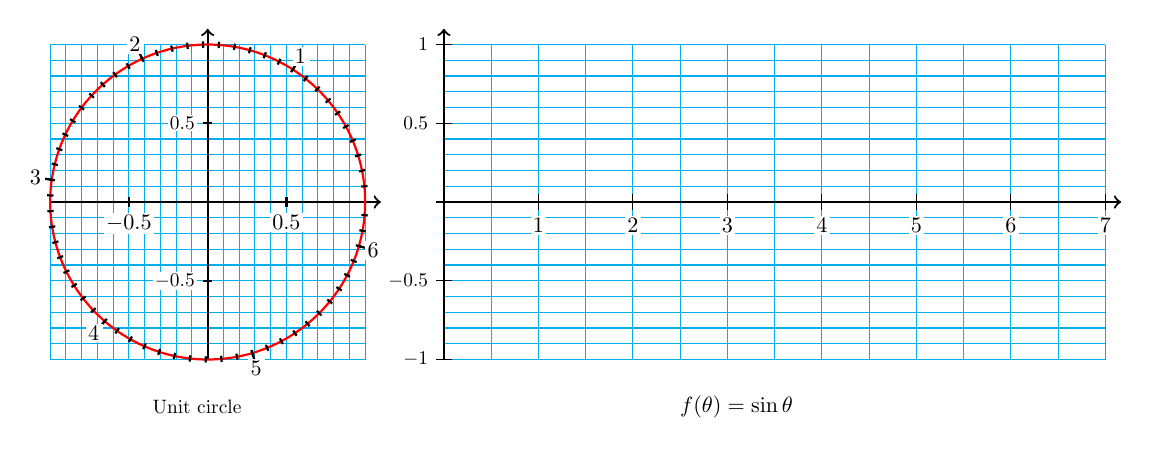
\begin{tikzpicture} [scale=2]

\draw[cyan] (-1.0001,-1.0001) grid[step = 0.1] (1,1);
\draw[black, thick, ->] (-1,0)--(1.1,0);
\draw[black, thick, ->] (0,-1)--(0,1.1);

\draw[red,thick] (0,0) circle (1cm);

\foreach \i in {0.1, 0.2, ..., 6.2} {
 \draw[black, thick] ({deg(\i)}:.98) -- ({deg(\i)}:1.02);
};
\foreach \i in {1,2, ..., 6} {
 \draw[black, thick] ({deg(\i)}:1) -- ({deg(\i)}:1.05);
 \node[text width=.2cm, fill=white, inner sep=1, scale=.8] at ({deg(\i)}:1.1) { $\i$};
};
\foreach \i in {-0.5, 0.5} {
 \draw[black, thick] (0.03,\i) -- (-0.03,\i) node[left, xshift=-2, fill=white, inner sep=1, scale=.7]{ $\i$};
 \draw[black, thick] (\i,0.03) -- (\i,-0.03) node[below, yshift=-2, fill=white, inner sep=1, scale=.8]{$\i$};
};

\node[text width=2cm, scale=.7] at (0,-1.3) {Unit circle};

%second grid
\draw[cyan] (1.4999,-1.0001) grid[xstep=.3, ystep=.1] (5.7,1);
\draw[black,thick,->] (1.45,0)--(5.8,0);
\draw[black,thick,->] (1.5,-1)--(1.5,1.1);

\foreach \x [evaluate=\x as \xi using (1.5 + .6* \x )]  in {1, 2,...,7}
 \draw[black] (\xi,.05)--++(0,-.1) node[below, yshift=-2, fill=white, inner sep =1, scale=.8] {$\x$};
 \foreach \y in {-1, -0.5, 0.5,1}
  \draw[black] (1.55,\y)--++(-.1,0) node[left, xshift=-2, fill=white, inner sep =1, scale=.7] {$\y$};

\node[text width=3cm, scale=.8] at (3.6,-1.3) {$ f(\theta) =\sin \theta $};

\end{tikzpicture}
\end{document}